\documentclass[a4paper,11pt]{report}
\usepackage[T1]{fontenc}
\usepackage[utf8]{inputenc}
\usepackage{lmodern}
\usepackage[brazilian]{babel}
\usepackage{amsfonts}
\usepackage{hyperref}
\usepackage{graphicx}
\usepackage{subcaption}
\usepackage{float}
\usepackage{amsmath}

\title{Relatório do projeto de MAC5768 - Visão e Processamento de Imagens}
\author{Rafael Reggiani Manzo}

\begin{document}

\maketitle
\tableofcontents

\begin{abstract}
  No início da disciplina foi proposto que este projeto consistisse de uma aplicação de processamento de imagens que agregue algo ao tema do meu mestrado. Então aqui será primeiro apresentado o problema de segmentação de imagens de ressonância magnética como uma das formas de mapear regiões de incerteza nestas.

  Em seguida, a solução pretendida por meio do algoritmo \textit{Watersheds} junto com a implementação feita em \textit{Python 3} serão detalhados para, por fim, os exibir os resultados obtidos que mostraram o algoritmo muito bom para pequenas regiões delimitadas, mas que para o todo da imagem produz tantas calhas que não é mais possível destinguir as regiões de incerteza das demais a olho nu, exigindo um algoritmo auxiliar na interpretação.
\end{abstract}

\chapter{Problema}
Aparelhos de ressonância magnética estão entre as mais versáteis ferramentas não invasivas de diagnóstico e estudo na área médica. Esses podem ser empregados tanto na aquisição de informações funcionais, como quais áreas do cérebro são ativadas para determinados estímulos, quanto para aquisição de informações estruturais, como reconstrução das fibras de substância branca do cérebro.

Sobre esta última modalidade mencionada, denominada \textit{Diffusion Tensor Imaging} (DTI) que iremos focar. Este é um tipo de imagem com quatro dimensões: três dimensões para a posição do voxel no espaço; e a última para uma matriz $3$x$3$ que quantifica a difusão da água no espaço (o tensor).

Porém, como a resolução das imagens adquiridas desta forma não possuem uma resolução tão alta, muitas vezes regiões de cruzamento entre fibras são representadas por um único voxel. Assim, não fornecendo a informação exata quanto a direcionalidade naquele ponto.

São tais pontos que constituem o que denominamos regiões de incerteza dentro da imagem. Então, o objetivo deste trabalho é mapear tais regiões.

A utilidade de tal mapa pode ir desde comparar imagens saudáveis com imagens que apresentem patologias até fornecer informações complementares para que algoritmos de reconstrução das fibras possam lidar melhor com este caso que ainda não é tratado por eles.

\chapter{Proposta}
O algoritmo de segmentação por \textit{Watersheds} é um dos mais clássicos para a segmentação de imagens. Uma boa implementação é descrita no artigo \textit{Vincent, Luc, and Pierre Soille. ``Watersheds in digital spaces: an efficient algorithm based on immersion simulations.'' IEEE transactions on pattern analysis and machine intelligence 13.6 (1991): 583-598.}.

Então, para este trabalho da disciplina de visão e processamento de imagens é o de implementar o algoritmo como é descrito no artigo, mas em três dimensões de forma a aplicá-lo na segmentação das regiões de incerteza supracitadas em uma imagem de ressonância magnética por tensor de difusão.

\chapter{Resultados}
  \section{Estudo do artigo}
  Uma imagem em escala de cinza pode ser encarada como se cada um de seus pixeis seja a elevação de um mapa topográfico. Desta forma, quando pensamos onde uma gota d'água pararia em certo ponto do mapa, teremos as divisões.

  Por outro lado, computar estas divisões seguindo esta linha de raciocínio é computacionalmente custoso e complicado de se implementar com precisão. Então, propõe-se imaginar que o mapa tenha furos em cada um de seus mínimos e esteja sendo mergulhado em água. Onde os fluxos d'água subindo se encontrarem temos as divisões. Constituindo assim, a abordagem ao algoritmo de segmentação Watersheds por imersão.

  Definir tal abordagem permite duas formas. Uma bastante teórica, útil para a compreensão de ideias básicas como calha (o conjunto de pixeis, cujo fluxo leva a um mínimo do mapa), e outra mais algorítmica mais adequada para o caso de funções digitais. Para essa segunda temos as seguintes definições prévias:

  \begin{itemize}
    \item Imagem: $I=\begin{cases}D_I \subseteq \mathbb{Z}^2 & \rightarrow \{0,...,N\} \\ p & \rightarrow I(p)\end{cases}$
    \item $h_{min}$: menor intensidade da imagem;
    \item $h_{max}$: maior intensidade da imagem;
    \item Threshold: $T_h(I) = \{ p \in D_I | I(p) \leq h\}$;
    \item $C_h(M) = C(M) \cap T_h(I)$;
    \item $d_A(x,y)$: tamanho do menor caminho no conjunto $A$ que liga os pontos $x$ e $y$, conhecido como distância geodésica.
  \end{itemize}

  Nesse mesmo conjunto $A$ da distância geodésica, suponhamos que existam $B_1,...,B_k$ componentes conexos. A zona de influência geodésica, $iz_A(B_i)$, de $B_i$ em $A$ é o conjunto de pontos cuja distância para $B_i$ é menor que a distância para todo $B_j$, $j \neq i$.

  $iz_A(B_i) = \{ p \in A | d_A(p, B_i) < d_A(p, B_j), \forall j \in [1, k] \setminus \{i\}\}$

  Pontos que não pertencem a nenhuma zona de influência são chamados esqueletos das zonas de influência.

  $SKIZ_A(B) = A \setminus iz_A(B)$

  Com a base definida, partimos para a descrição da simulação do processo de imersão que se inicia com:

  $X_{h_{min}} = T_{h_{min}}(I)$

  Consideremos $T_{h_{min} + 1}(I) \supseteq X_{h_{min}}$ e $Y$ uma de suas componentes conexas, temos as seguintes relações de inclusão entre $X_{h_{min}} \cap Y$ e $Y$:

  \begin{enumerate}
    \item Se $X_{h_{min}} \cap Y = \emptyset$, então $Y$ é um novo mínimo de $I$;
    \item Se $X_{h_{min}} \cap Y \neq \emptyset$ e é conexo, então $Y$ corresponde exatamente aos pixeis da calha associada ao mínimo $X_{h_{min}} \cap Y$ com nível inferior a $h_{min} + 1$;
    \item Se $X_{h_{min}} \cap Y \neq \emptyset$ e é desconexo, então $Y$ contém mínimos diferentes de $I$, $Z_1,...,Z_k$, com $C_{h_{min} + 1}(Z_i) = iz_Y(Z_i)$.
  \end{enumerate}

  Então para cada nível valem estas relações dadas previamente para $X_{h_{min} + 1} = min_{h_{min}+1} \cup IZ_{T_{h_{min} + 1}(I)}(X_{h_{min} + 1})$

  Assim, o conjunto de calhas da imagem I é igual ao conjunto $X_{h_{max}}$ obtido pela recursão:

  \begin{enumerate}
    \item $X_{h_{min}} = T_{h_{min}}(I)$
    \item $X_{h_{min} + 1} = min_{h_{min}+1} \cup IZ_{T_{h_{min} + 1}(I)}(X_{h_{min} + 1})$
    \item E as divisórias por $D_I \setminus X_{h_{max}}$
  \end{enumerate}

  Além do algoritmo a ser proposto logo a seguir, já existem outras implementações cada uma com suas vantagens e desvantagens para esta ideia de imersão: grossura das divisas; esqueletos de tons de cinza; até implementações sequenciais.

  O algoritmo proposto baseia-se em dois passos principais: ordenação e inundação. A primeira baseia-se em um algoritmo com consumo de tempo $O(2N)$ que calcula as frequências relativas e então as acumula para, por fim, com esta informação atribui os pixeis de forma ordenada às devidas células de um vetor.

  Em seguida, a inundação parte de um nível $h$ até o qual já foi feita a inundação e as calhas estão devidamente marcadas unicamente. Então, no nível $h + 1$ a todos os pixeis é atribuída uma marcação de máscara, todos que forem vizinhos de pixeis já marcados são colocados em uma fila para um a um estenderem as calhas de acordo com as zonas de influência geodésica. Após isto, apenas os novo mínimos em $h + 1$ ainda estão marcados com a máscara. Esta fila é importante para solucionar os problemas de precisão encontrados em outros algoritmos.

  Fazendo a suposição da possibilidade de estruturas de acesso direto à posições aleatórias de memória, ele fornece complexidade de processamento e consumo de memória lineares na quantidade de pixeis.

  Este artigo possui diversos pontos fortes: explicação didática, proposta de um algoritmo inovador em termos de eficiência, exemplos ilustrados e casos de uso. Realmente muito completo e bem escrito. Talvez seu ponto fraco seja a ausência de uma descrição mais detalhada para o problema em três dimensões que hoje é um domínio com interesse muito grande.

  \section{Descrição da implementação}
  O algoritmo de \textit{Watersheds} foi implementado em \textit{Python 3}. Ele encontra-se dentro do código entregue junto com este relatório na pasta:

  \textit{dti-tools/src/classes/watershed\_segmentation\_step.py}

  E também em:

  \url{https://github.com/rafamanzo/dti-tools/blob/master/src/classes/watershed_segmentation_step.py}.

  Assim, portanto, vale dizer que ele está junto a diversos outros algoritmos já implementados por mim para atingir o objetivo deste trabalho.

  No que diz respeito, a mudança do algoritmo de duas dimensões descrito no artigo para três dimensões foi bastante simples, apenas necessitando modificar a função auxiliar que dá os vizinhos de um determinado voxel.

  \section{Testes}
    Como o algoritmo de \textit{Watersheds} espera que os dados da imagem estejam em escala de cinza ou ao menos em alguma escala de inteiros, para os testes foi preciso antes realizar transformações sobre a imagem:

    \begin{enumerate}
      \item Mapa de anisotropia fracionária
      \item Discretização do mapa
    \end{enumerate}

    O primeiro passo quantifica a informação de cada voxel em um índice bastante usado na análise destas imagens, conhecido como anisotropia fracionária. Com valores reais enter 0 e 1, esse índice quantifica o quão um tensor é anisotrópico (valor 1 para anisotropia perfeita, ou o que chamamos de certeza quanto a direção) ou isotrópico (valor 0 para isotropia perfeita, ou o que chamamos de incerteza quanto a direção).

    Por fim, o segundo vai multiplicar tal valor de 0 a 1 por 100 e então pegar o chão do resultado a fim de finalmente se ter uma escala de inteiros como é pretendido.

    \subsection{Pequena região}
    A região foi selecionada aplicando um algoritmo de reconstrução de fibras no \textit{corpus callosum} do cérebro. Esta é uma região de interconexão enter os diferentes hemisférios do cérebro e portanto de onde muitas fibras partem.

    Nessa reconstrução foi selecionada uma pequena região onde sabemos que o algoritmo de reconstrução falhou devido à incerteza e então foi aplicado o algoritmo de segmentação sobre esta região.

    \begin{figure}[H]
      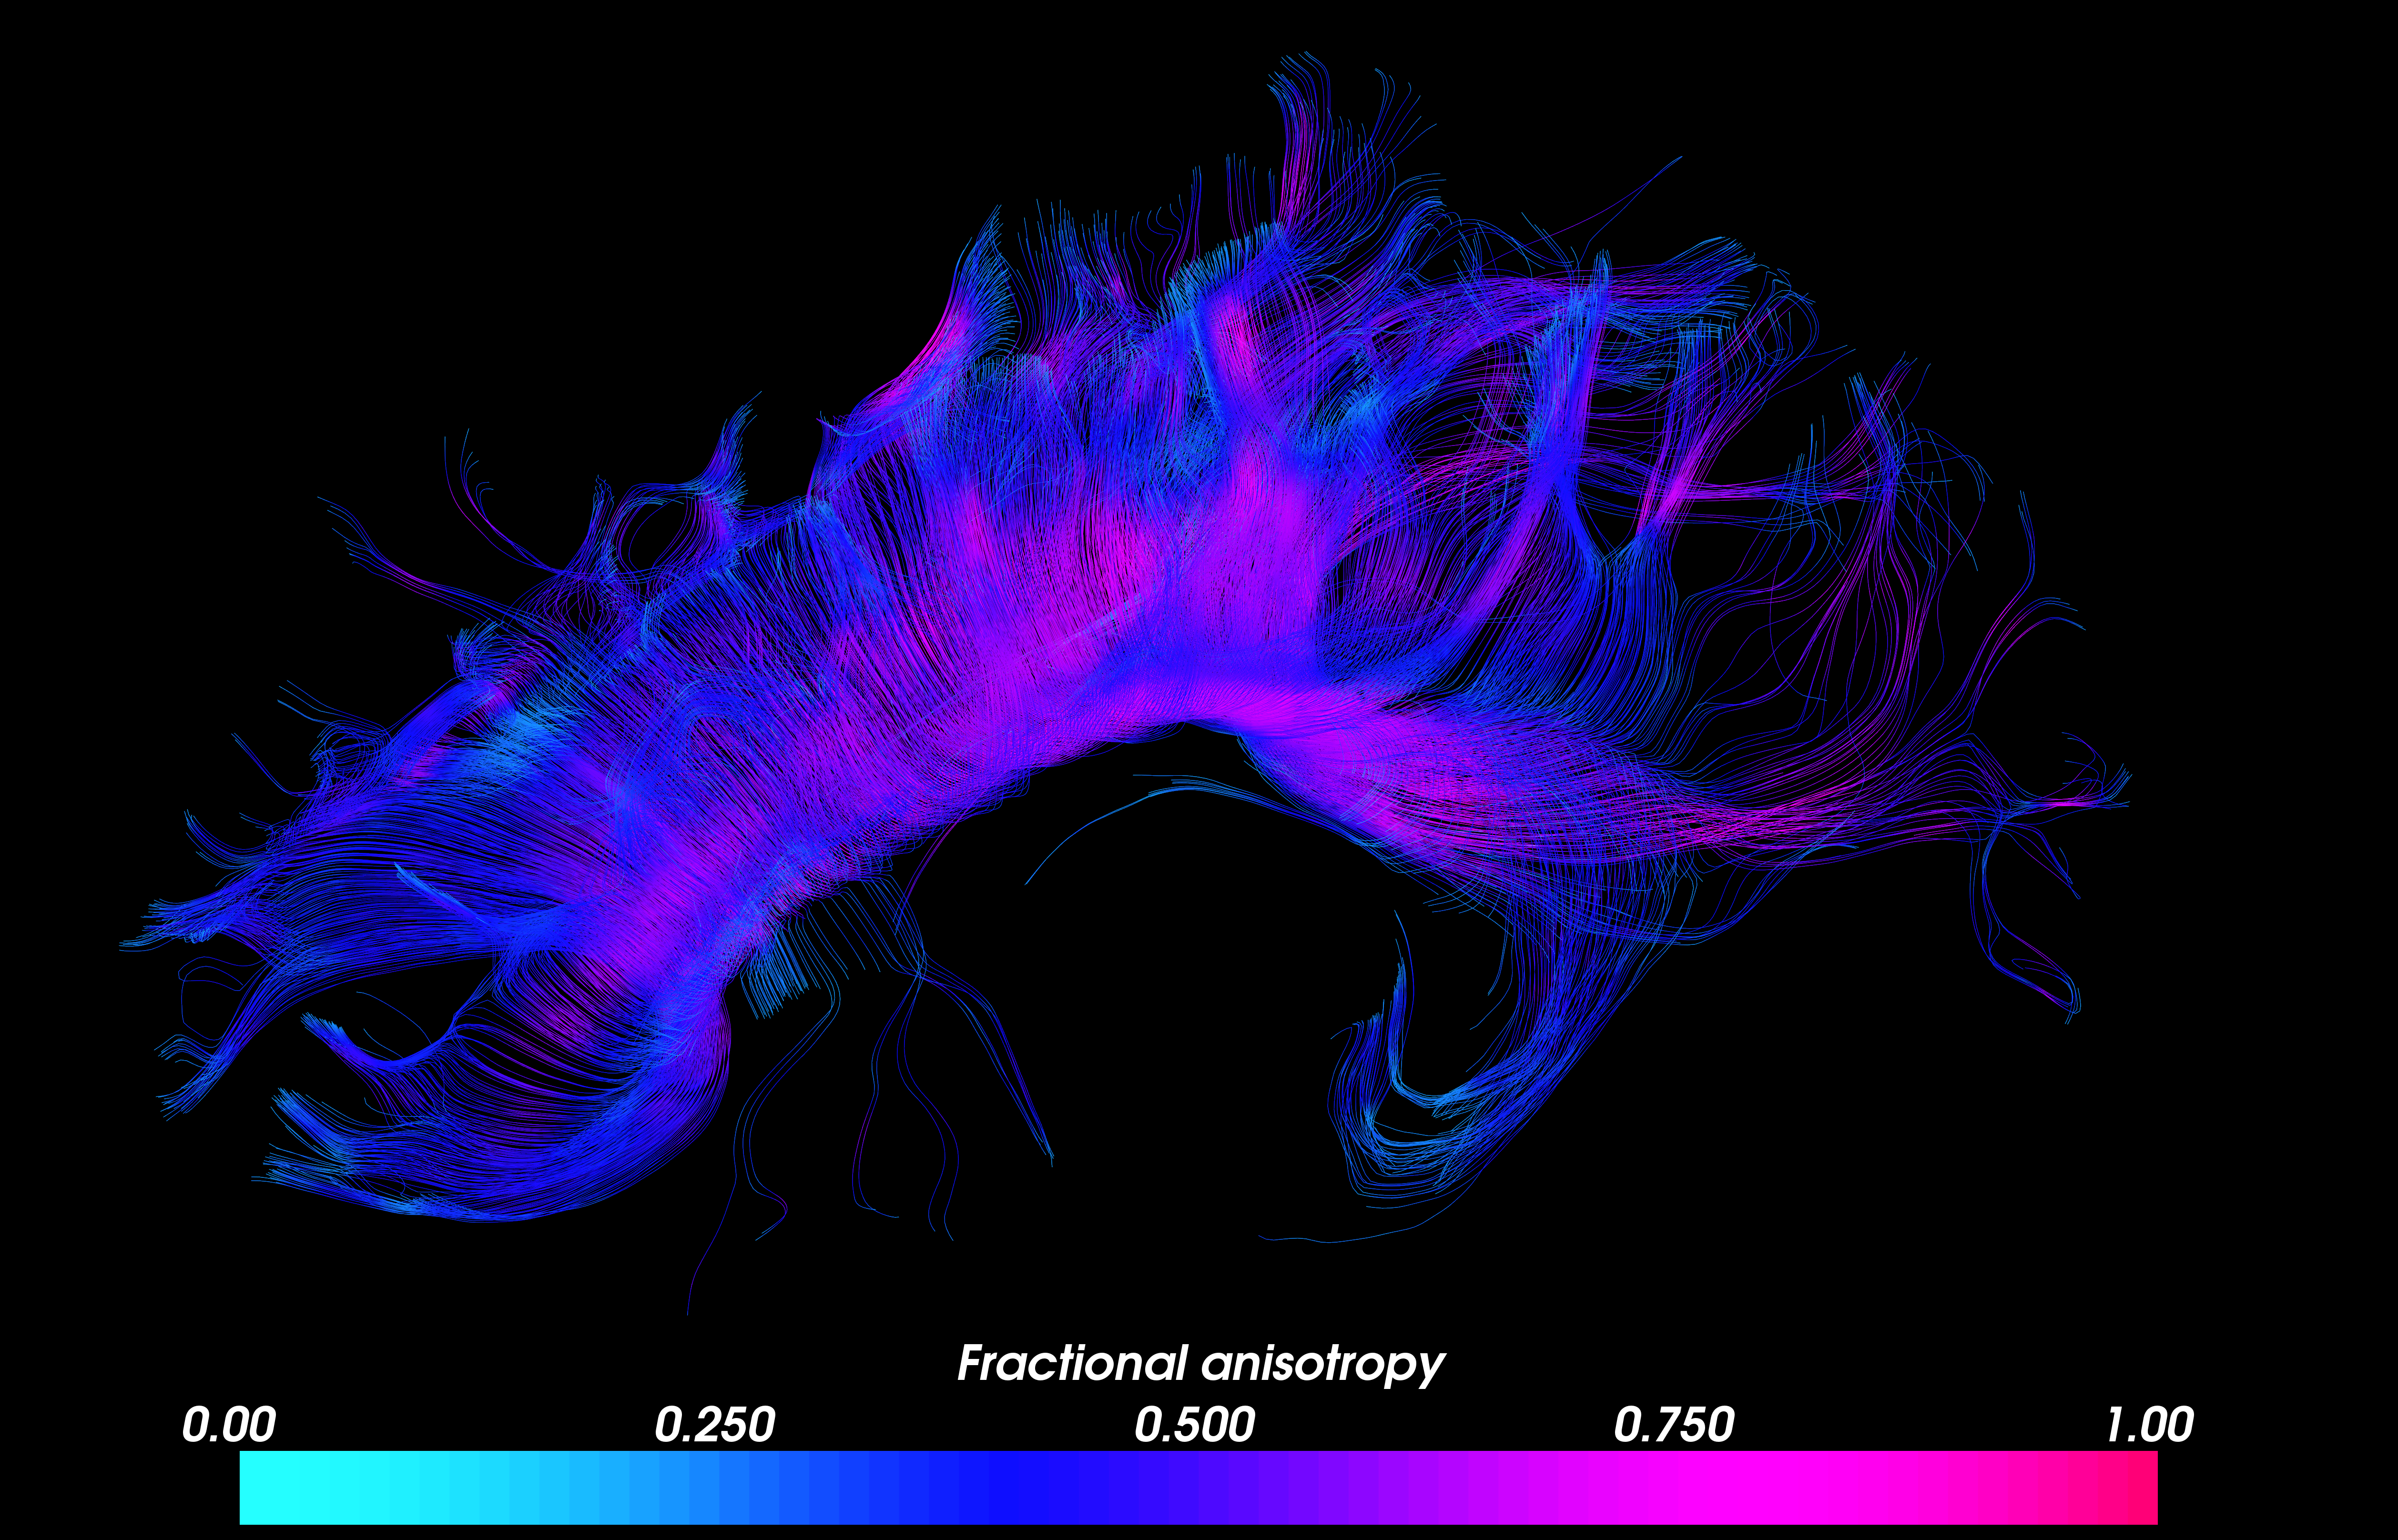
\includegraphics[width=1\linewidth]{imgs/cc-expanded-fibers.png}
      \caption{Visualização em 3D do \textit{corpus callosum} com a tractografia aplicada pelo método de Runge-Kutta adaptativo no software Bio Image Suite.}
      \label{fig:fibres}
    \end{figure}

    \begin{figure}[H]
      \includegraphics[width=1\linewidth]{imgs/cc-expanded-fibers-mask.png}
      \caption{Visualização em 3D do \textit{corpus callosum} com a tractografia aplicada pelo método de Runge-Kutta adaptativo no software Bio Image Suite combinada com a máscara gerada para todas as fibras}
      \label{fig:fibres-mask}
    \end{figure}

    \begin{figure}[H]
      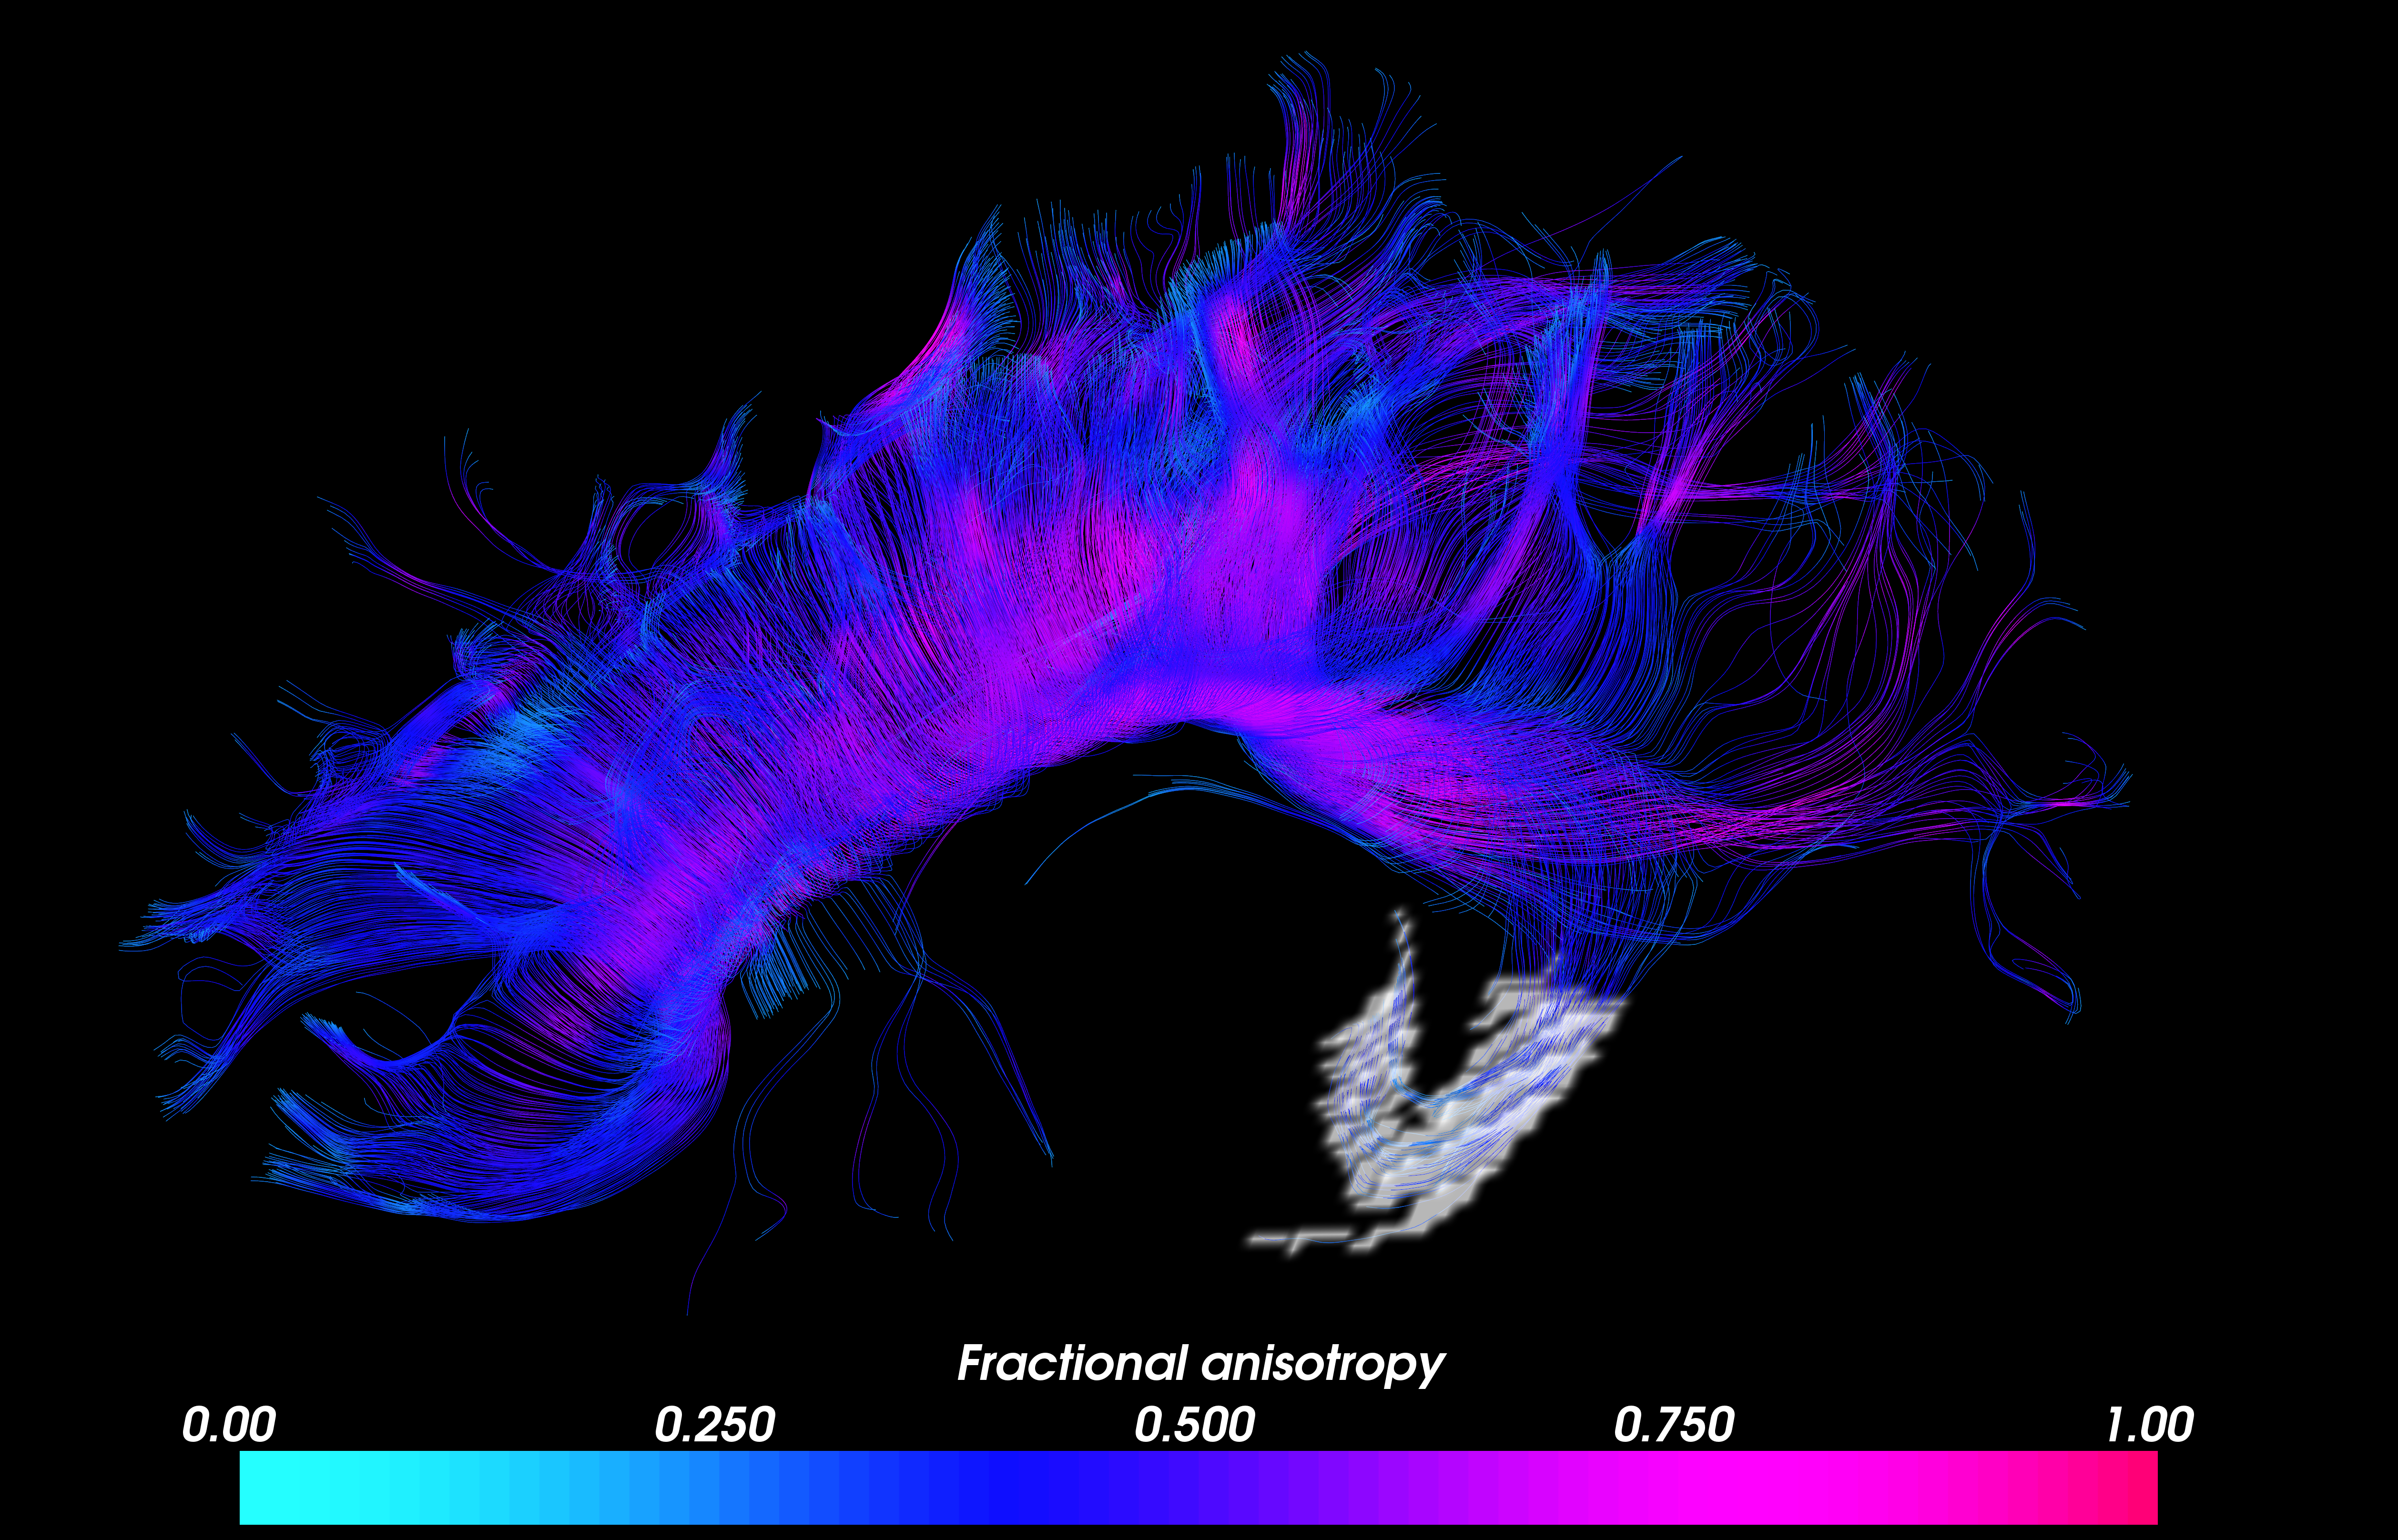
\includegraphics[width=1\linewidth]{imgs/cc-expanded-fibers-mask-croped.png}
      \caption{Visualização em 3D do \textit{corpus callosum} com a tractografia aplicada pelo método de Runge-Kutta adaptativo no software Bio Image Suite combinada com a máscara gerada para todas as fibras recortada na região de interesse}
      \label{fig:fibres-mask-croped}
    \end{figure}

    \begin{figure}[H]
      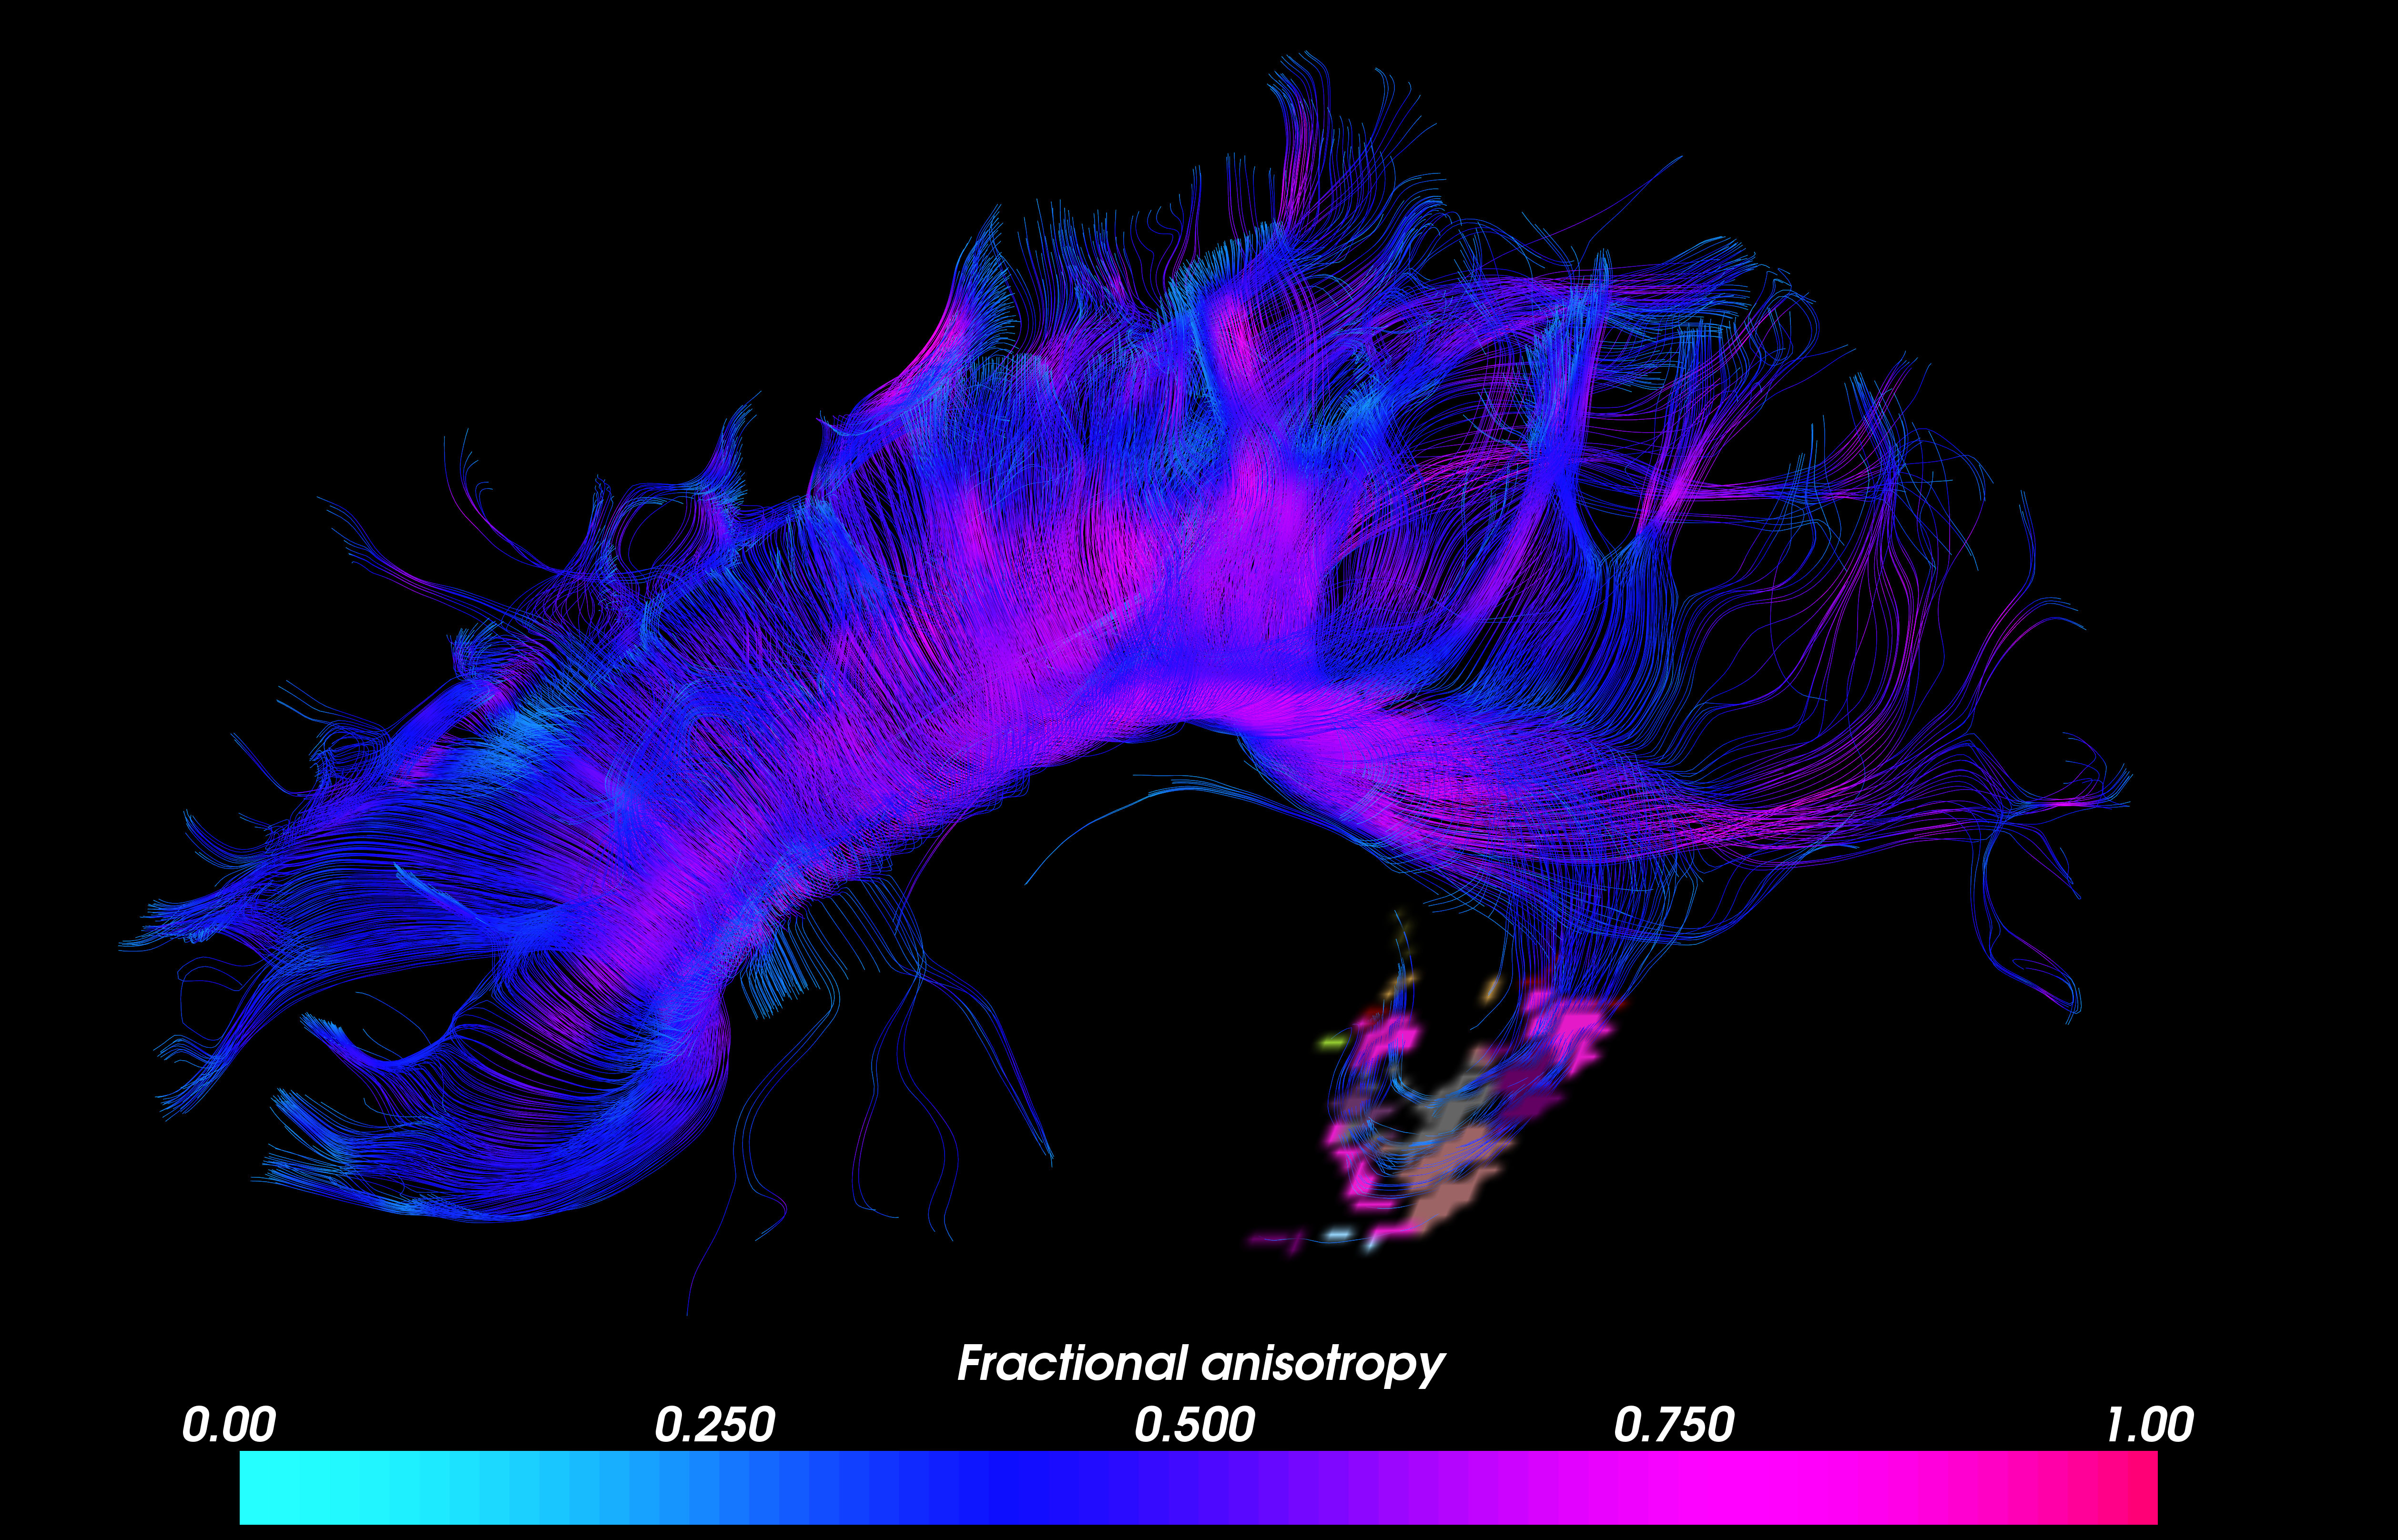
\includegraphics[width=1\linewidth]{imgs/cc-expanded-fibers-mask-croped-watersheds.png}
      \caption{Visualização em 3D do \textit{corpus callosum} com a tractografia aplicada pelo método de Runge-Kutta adaptativo no software Bio Image Suite combinada com a máscara gerada para todas as fibras recortada na região de interesse e então segmentado}
      \label{fig:fibres-mask-croped-segmented}
    \end{figure}

    Para uma melhor comparação da região original com a segmentada podemos ver lado a lado o zoom das imagens na região de interesse:

    \begin{figure}[H]
      \centering
      \begin{subfigure}[t]{.49\textwidth}
        \includegraphics[width=1\linewidth]{imgs/cc-expanded-fibers-mask-croped-zoomed.png}
        \caption{Interest region zoom}
        \label{subfig:fibres-mask-croped-zoomed}
      \end{subfigure}\hfill%
      \begin{subfigure}[t]{.49\textwidth}
        \includegraphics[width=1\linewidth]{imgs/cc-expanded-fibers-mask-croped-watersheds-zoomed.png}
        \caption{Interest region segmented zoom}
        \label{subfig:fibres-mask-croped-segmented-zoomed}
      \end{subfigure}\hfill
    \end{figure}

    É possível notar que a região em cinza engloba exatamente onde as fibras fazem a curva fechada que, por sua vez, pode ser entendida como a regão de incerteza.

    \begin{figure}[H]
      \centering
      \includegraphics[width=0.6\linewidth]{imgs/cc-expanded-fibers-mask-croped-watersheds-region7-zoomed.png}
      \caption{Ampliação da região segmentada isolada.}
      \label{fig:fibres-mask-croped-segmented-region}
    \end{figure}

  \subsection{Aplicando para todo o conjunto de dados}
  Infelizmente, para um conjunto grande de dados, aconteceu exatamente o previsto pelo artigo: um conjunto muito grande de calhas segmentadas:

  \begin{figure}[H]
    \includegraphics[width=1\linewidth]{imgs/fa_watersheds.png}
    \caption{Corte sagital em (70, 70, 48) para os \textit{Watersheds} de FA.}
    \label{fig:fa_watersheds}
  \end{figure}

  Porém um algoritmo de crescimento de regiões como sugerido parece promissor

  \begin{figure}[H]
    \includegraphics[width=1\linewidth]{imgs/fa_watersheds_01_20_grown.png}
    \caption{Corte sagital em (70, 70, 48) para os \textit{Watersheds} de FA crescidos.}
    \label{fig:fa_watersheds_grown}
  \end{figure}

\chapter{Conclusão}
Uma vez lido o artigo e compreendido, fica muito simples a implementação do algoritmo seguindo sua descrição. Então a aplicação do algoritmo trouxe surpresas positivas para um caso pequeno e controlado, mas, por outro lado, gerou preocupação quando aplicado a uma região grande onde diversos casos se misturam. Como era previsto um algoritmo de crescimento de regiões (que precisa ser melhorado) é necessário em conjunto nesse caso.

\end{document}